\documentclass[border=8pt]{standalone}
\usepackage{tikz}
\usetikzlibrary{positioning, arrows.meta, fit, calc, backgrounds}

\definecolor{coreblue}{HTML}{2563EB}
\definecolor{surfgreen}{HTML}{16A34A}
\definecolor{reachpurple}{HTML}{9333EA}
\definecolor{estorange}{HTML}{EA580C}
\definecolor{ctrlred}{HTML}{DC2626}
\definecolor{plantbrown}{HTML}{92400E}
\definecolor{archgray}{HTML}{475569}
\definecolor{benchgold}{HTML}{CA8A04}
\definecolor{lightbg}{HTML}{F8FAFC}

\begin{document}
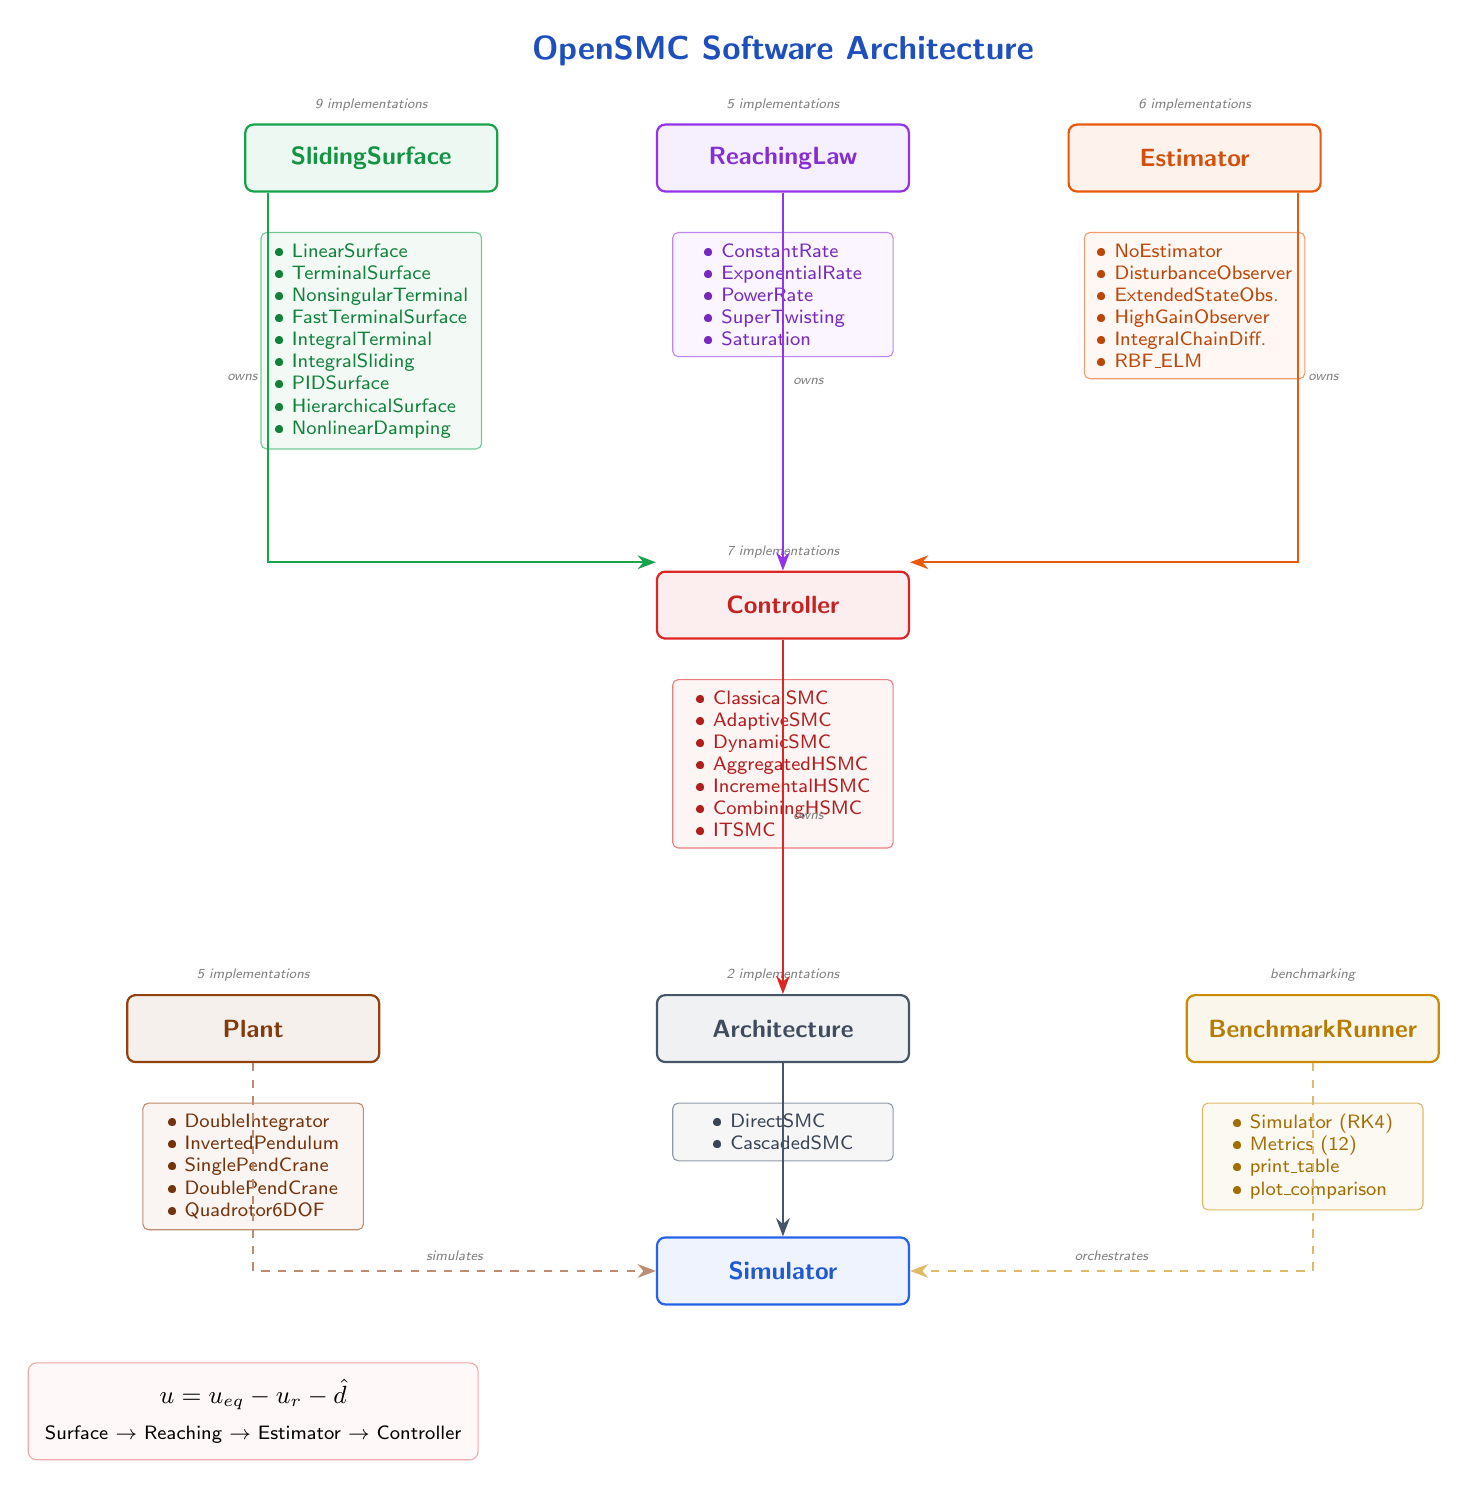
\begin{tikzpicture}[
    >=Stealth,
    node distance=1.2cm and 1.6cm,
    interface/.style={
        rectangle, draw=#1, thick, fill=#1!8, rounded corners=3pt,
        minimum width=3.2cm, minimum height=0.85cm,
        font=\sffamily\small\bfseries, text=#1!90!black, align=center
    },
    impl/.style={
        rectangle, draw=#1!60, fill=#1!5, rounded corners=2pt,
        minimum width=2.8cm, font=\sffamily\scriptsize, text=#1!80!black,
        align=left, inner sep=4pt
    },
    comp/.style={->, thick, #1},
    uses/.style={->, dashed, thick, #1!60},
    label/.style={font=\sffamily\tiny\itshape, text=gray}
]

%% ---- Row 1: Components owned by Controller ----

% Sliding Surface
\node[interface=surfgreen] (surf) {SlidingSurface};
\node[impl=surfgreen, below=0.5cm of surf] (surf_impl) {%
    \textbullet~LinearSurface\\
    \textbullet~TerminalSurface\\
    \textbullet~NonsingularTerminal\\
    \textbullet~FastTerminalSurface\\
    \textbullet~IntegralTerminal\\
    \textbullet~IntegralSliding\\
    \textbullet~PIDSurface\\
    \textbullet~HierarchicalSurface\\
    \textbullet~NonlinearDamping%
};
\node[label, above=1pt of surf] {9 implementations};

% Reaching Law
\node[interface=reachpurple, right=2.0cm of surf] (reach) {ReachingLaw};
\node[impl=reachpurple, below=0.5cm of reach] (reach_impl) {%
    \textbullet~ConstantRate\\
    \textbullet~ExponentialRate\\
    \textbullet~PowerRate\\
    \textbullet~SuperTwisting\\
    \textbullet~Saturation%
};
\node[label, above=1pt of reach] {5 implementations};

% Estimator
\node[interface=estorange, right=2.0cm of reach] (est) {Estimator};
\node[impl=estorange, below=0.5cm of est] (est_impl) {%
    \textbullet~NoEstimator\\
    \textbullet~DisturbanceObserver\\
    \textbullet~ExtendedStateObs.\\
    \textbullet~HighGainObserver\\
    \textbullet~IntegralChainDiff.\\
    \textbullet~RBF\_ELM%
};
\node[label, above=1pt of est] {6 implementations};

%% ---- Row 2: Controller ----
\node[interface=ctrlred, below=4.8cm of reach] (ctrl) {Controller};
\node[impl=ctrlred, below=0.5cm of ctrl] (ctrl_impl) {%
    \textbullet~ClassicalSMC\\
    \textbullet~AdaptiveSMC\\
    \textbullet~DynamicSMC\\
    \textbullet~AggregatedHSMC\\
    \textbullet~IncrementalHSMC\\
    \textbullet~CombiningHSMC\\
    \textbullet~ITSMC%
};
\node[label, above=1pt of ctrl] {7 implementations};

% Composition arrows (Controller owns Surface, ReachingLaw, Estimator)
\draw[comp=surfgreen]   (surf.south west) ++(0.3, 0) |- ([yshift=3pt]ctrl.north west) node[pos=0.25, left, label] {owns};
\draw[comp=reachpurple]  (reach) -- (ctrl) node[midway, right, label] {owns};
\draw[comp=estorange]   (est.south east) ++(-0.3, 0) |- ([yshift=3pt]ctrl.north east) node[pos=0.25, right, label] {owns};

%% ---- Row 3: Architecture ----
\node[interface=archgray, below=4.5cm of ctrl] (arch) {Architecture};
\node[impl=archgray, below=0.5cm of arch] (arch_impl) {%
    \textbullet~DirectSMC\\
    \textbullet~CascadedSMC%
};
\node[label, above=1pt of arch] {2 implementations};

% Architecture owns Controller(s)
\draw[comp=ctrlred] (ctrl) -- (arch) node[midway, right, label] {owns};

%% ---- Plant (to the left) ----
\node[interface=plantbrown, left=3.5cm of arch] (plant) {Plant};
\node[impl=plantbrown, below=0.5cm of plant] (plant_impl) {%
    \textbullet~DoubleIntegrator\\
    \textbullet~InvertedPendulum\\
    \textbullet~SinglePendCrane\\
    \textbullet~DoublePendCrane\\
    \textbullet~Quadrotor6DOF%
};
\node[label, above=1pt of plant] {5 implementations};

%% ---- Benchmark (to the right) ----
\node[interface=benchgold, right=3.5cm of arch] (bench) {BenchmarkRunner};
\node[impl=benchgold, below=0.5cm of bench] (bench_impl) {%
    \textbullet~Simulator (RK4)\\
    \textbullet~Metrics (12)\\
    \textbullet~print\_table\\
    \textbullet~plot\_comparison%
};
\node[label, above=1pt of bench] {benchmarking};

% Simulator in the middle
\node[interface=coreblue, below=2.2cm of arch] (sim) {Simulator};

% Connections
\draw[comp=archgray]    (arch) -- (sim) node[midway, right, label] {};
\draw[uses=plantbrown]  (plant) |- (sim) node[pos=0.75, above, label] {simulates};
\draw[uses=benchgold]   (bench) |- (sim) node[pos=0.75, above, label] {orchestrates};

%% ---- Control law formula ----
\node[draw=ctrlred!40, fill=ctrlred!3, rounded corners=3pt,
      font=\small, inner sep=6pt, align=center,
      below=3.8cm of plant] (formula) {%
    $u = u_{eq} - u_r - \hat{d}$\\[2pt]
    {\scriptsize\sffamily Surface $\to$ Reaching $\to$ Estimator $\to$ Controller}
};

%% ---- Title ----
\node[font=\sffamily\large\bfseries, text=coreblue!80!black,
      above=0.6cm of reach] {OpenSMC Software Architecture};

\end{tikzpicture}
\end{document}
